\documentclass[twocolumn,nofootinbib,notitlepage,aps]{revtex4-1}
\usepackage{amsmath}
\usepackage{amssymb}
\usepackage{graphicx}
\usepackage{lmodern}
\usepackage[T1]{fontenc}
\usepackage{textcomp}


\begin{document}
\title{High Speed in situ X-ray Diffraction Characterization of Temperature and Phase Fractions in Cold Metal Transfer Welded Stainless Steel 308L}
\author{Nathan S. Johnson}
\affiliation{Department of Mechanical Engineering, Colorado School of Mines}
\affiliation{Los Alamos National Laboratory}

\author{Donald W. Brown}
\affiliation{Los Alamos National Laboratory}

\author{Aaron P. Stebner}
\affiliation{Department of Mechanical Engineering, Georgia Technical Institute}

\author{Craig A. Brice}
\affiliation{Department of Mechanical Engineering, Colorado School of Mines}


\begin{abstract}
abstract goes here
\end{abstract}

\maketitle

\section{Introduction}
Modern manufacturing techniques like additive manufacturing (AM) are increasingly requiring methods of performing in situ characterization that can elucidate important thermodynamic information about the solidification process such as temperatures inside the weld, cooling rates, phase fractions, and more. The nature of additive manufacturing makes such characterization difficult. The small melt pools observed in AM make traditional in situ monitoring techniques, like thermography or two-color pyrometry, difficult to implement and analyze. Furthermore, these traditional techniques can rarely probe the internal structure of the weld pool where the most dynamic behavior is occurring. 

Everton et al. provide a comprehensive review of in situ monitoring techniques applied to metal AM through 2016 \cite{Everton2016}. Many of the studies cited in \cite{Everton2016} focus on detection and mitigation of defects during the manufacturing process. Many studies used on-line optical or thermal cameras during manufacturing to measure melt pool properties such as temperature \cite{Zalameda2013, Liu2014} and melt pool morphology \cite{Li2018}. More recent studies have implemented systems like acoustic sensing to detect pore formation \cite{Shevchik2018}.

As noted in \cite{Everton2016} there is significant industrial push for in situ monitoring and measurement techniques for the additive process. However, in situ monitoring techniques must be validated and compared against known values for relevant properties. Furthermore, many of the studies cited above are surface measurements of the melt pool and cannot probe the internal behavior of the manufacturing process.

Brown et al. recently developed a technique for measurement of temperature inside weld pools using high energy X-ray diffraction \cite{Brown2019}. Brown measured lattice strains as cold metal transfer (CMT) welds of 308L stainless steel solidified on a stainless substrate. These strains were then correlated with temperature based on macroscopic measurements of strain in bulk SS 308L as a function of temperature \cite{Touloukian1975}. Brown validated these temperature measurements using a finite element model of the same geometry cooling on a substrate. This bulk measurement technique is taken in transmission through the sample providing measurements of temperature inside the weld as it is cooling. However, the study of Brown et al. used a fairly slow data acquisition rate that may not have been able to fully capture the dynamics of the solidification process. 

In this study, the technique of Brown et al. is expanded upon to characterize the cooling of SS 308L CMT welds during the solidification process at a data acquisition rate of 200 Hz. Furthermore, a first-order model is developed to characterize phase fractions of the liquid, ferrite, and austenite phases during the solidification process.

%%%%%%%%%%%%%%%%%%%%%%%%%%%%%%%%%%
\section{Methods}

\begin{figure*}
	\includegraphics[width=0.75\linewidth]{weld_setup}
	\caption{A graphic depiction of the in situ diffraction welder experiment.}
	\label{weldsetup}
\end{figure*}
A schematic of the in situ diffraction welder setup can be seen in Figure \ref{weldsetup}. Single beads of stainless steel 308L were deposited onto a stainless steel 304L water cooled substrate. Weld deposits were made using a Fr\"onius Cold Metal Transfer welder. Each weld deposit was approximately 2.5mm in width and 2.5mm in height. 

X-ray diffraction experiments were performed at the 1ID beamline of the Advanced Photon Source, Argonne National Laboratory. A 71 keV, $100\mu$m $\times 100 \mu$m box beam was used. As samples were being deposited the X-ray beam was shone on the liquid sample. Data was collected through deposition and until the beads were fully solidified. Data was collected using a dual-detector setup. One detector was and ASI Lynx detector \cite{LynX} with a refresh rate of 200 Hz and a small azimuthal coverage in the diffraction cone. The other detector was a GE detector with a refresh rate of 10 Hz and an azimuthal coverage of around 180 degrees. 

The use of multiple detectors was twofold. The ASI detector had a significantly higher refresh rate and therefore could capture dynamics of the solidification process which may be unobtainable using the slower GE detector. However, the ASI detector's small azimuthal range meant that grain statistics may be too few to accurately observe and measure the phase fractions of each phase. Thus, the ASI detector was used for calculations of strains from the grains which were detected and the GE detector was used to compare grain statistics with the ASI detector. In the end, it was found that the grain statistics were high enough on the ASI detector to trust phase fraction calculations. Thus, phase fraction changes were measured using the ASI detector and double-checked with the GE detector to ensure accuracy.

Data was collected at several locations throughout the welds -- 0.4mm, 0.8mm, and 1.2mm above the build substrate. Since data could only be collected at one location at a time, multiple welds were characterized at each location. This was done to see if differences in cooling rate could be observed throughout the sample.

After deposition weld beads were cut from the substrate and EBSD microscopy was performed. An example EBSD image can be seen in Figure \ref{EBSD}. The grain size distribution and orientation changes significantly from bottom to top of the weld bead. At the bottom, near the substrate, the grains are mostly equiaxed and have a fairly random distribution. The grain size ranges from single to tens of microns. Near $0.4$mm the grain structure changes to lamellar grains with a major axis in the hundreds of microns. A similar change can be observed at the side of the sample between 0.1mm and 0.4mm. The change in grain size is associated with a changing cooling rate during solidification. The weld bead likely nucleated grains rapidly in the center of the weld at first. At solidification continued and the mass of the sample grew the cooling rate slowed allowing for growth dominated grain formation.

\begin{figure}
	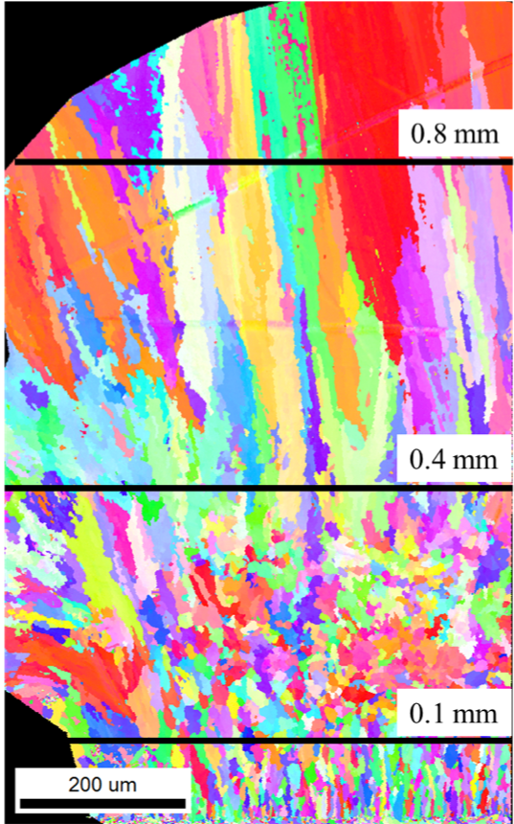
\includegraphics[width=1\linewidth]{SS_EBSD_weldbead}
	\caption{Electron Backscatter Diffraction image of one of the stainless steel weld beads, reprinted from Brown et al. \cite{Brown2019}.}
	\label{EBSD}
\end{figure}

Data was analyzed using the General Structure Analysis Software II (GSASII) \cite{GSASII}. Data was fully integrated on both detectors in order to provide maximal intensity and coverage for analysis. The first 1000 images of the ASI detector were analyzed while the full dataset for the GE detector, 120 images, were analyzed. The first 1000 images of the ASI were analyzed because data was repetitious after that point and the number of images taken was too large to be analyzed in a reasonable amount of time. 

The background function of the data needed to be fit in order to analyze the X-ray scattering through the liquid phase. The amorphous phase scattering can be described by the theory of Guinier explained in Section \cite{Guinier1994}. X-ray scattering through a liquid is analogous to scattering by an ideal gas, where the pair correlation function, which is dependent on density, determines the scattering length and intensity of the X-rays. A Gaussian function was fit to the background to capture the dynamics of the amorphous phase. The integrated intensity of the background Gaussian function was used to characterize the amount of liquid in the sample. Diffraction locations were refined in GSASII from the first peak with reasonable intensity and breadth. 

Rietveld refinement was used to fit the lattice parameters and intensity of the two phases of the SS308L, the ferrite ($\delta$) and austenite ($\gamma$) phases. The phase fraction of the liquid, ferrite, and austenite phases was fit by using
\begin{equation}
	f_{p} = \frac{p}{\delta_i + \gamma_i + A*B_i}
	\label{phasefrac}
\end{equation}
where $f_{p}$ is the scale factor of the phase being calculated, $\delta_i$ is the intensity of the ferrite phase at time $i$, $\gamma_i$ is the intensity of the austenite phase at time $i$, $B_i$ is the intensity of the Gaussian function fit to the background at time $i$, and $p = \delta_i$, $\gamma_i$, or $B_i$. The prefactor $A$ is a multiplier to scale the background function to the same magnitude as the intensity of the phases. 

To calculate temperature, the strain in the austenite phase had to be calculated. The austenite lattice parameter in the last frame obtained was used as a datum. Strain at each time step $\epsilon_i$ was calculated as
\begin{equation}
	\epsilon_i  = \frac{a_i - a_\infty}{a_\infty}
	\label{strain}
\end{equation}
where $a$ is the austenite lattice parameter found using Rietveld refinement, $a_i$ is the lattice parameter at time step $i$ and $a_\infty$ is the lattice parameter in the final image when the sample had sufficient time to cool off and relax.

Temperature measurements were made by fitting the lattice parameter expansion during cooling to the thermal expansion of SS308L as reported by Touloukian et al. \cite{Touloukian1975}. The fit is given by
\begin{equation}
\begin{split}
	\epsilon_i & = -0.358 + (9.472\times10^{-4})T_i + \\
	& (1.031\times10^{-6})T_i^2 - (2.978\times10^{-10})T_i^3\\
	\label{touloukian}
	\end{split}
\end{equation}
where $T_i$ is the temperature at time $i$. Equation \ref{touloukian} was fit using the \textbf{roots()} function in the scipy\textunderscore optimize python package. Equation \ref{touloukian} was modified to be 

\begin{equation}
\begin{split}
	0 & = -0.358 + (9.472\times10^{-4})T_i + \\
	& (1.031\times10^{-6})T_i^2 - (2.978\times10^{-10})T_i^3 - \epsilon_i\\
	\label{zeros}
	\end{split}
\end{equation}
and the polynomial roots were found. The roots were then used to find values of $T_i$ at every $\epsilon_i$. 




%%%%%%%%%%%%%%%%%%%%%%%%%%%%%%
\section{Results}
The raw scale factors obtained from X-ray diffraction can be seen in Figure \ref{scale}. Initially, when the weld is still liquid on the substrate no diffraction peaks can be observed for either the ferrite or austenite phases. As the temperature drops below the liquidus peaks begin to appear in the diffraction histogram. The phase diagram for SS 308L has a very small three-phase region of liquid, ferrite and austenite, with the liquidus being around 1455$^\circ$ C and the solidus at 1400$^\circ$ C \cite{matweb}. Due to the small solidification range the liquid background peak, ferrite peak, and austenite peaks are observed simultaneously very briefly.

There was a brief dip in the austenite peak intensities around 2.5 seconds that has not yet been explained. The same behavior was not observed for the ferrite phase.

Figure \ref{phasefraction} shows the phase fractions of the liquid, ferrite, and austenite phases. The sample is entirely liquid from the point of deposition through around 2s into welding. The three phases are briefly observed together as the liquid background peak transitions to zero and the intensity of the solid peaks grows. It should be noted that the liquid phase fraction changes rapidly at first but does not scale exactly to zero when the ferrite and austenite peaks grow. There was some residual amorphous background scattering that occurred. This is likely due to the changing cooling rate in the sample. Because the sample solidified from the center first it is likely that there was some solid crystallite diffraction occurring in the center at the same time as amorphous liquid scattering from the edge. This is a downside of transmission diffraction through bulk samples -- it is not possible to resolve where the sources of various scattering occurred in the sample. However, since the sample was simultaneously solid and liquid the phase fraction calculation makes sense, as it accurately quantified the amount of each phase based on the intensity of the X-ray scattering. There is a brief spike in the ferrite phase fraction initially until it eventually levels off and settles at around 10\% retained ferrite. The remaining diffraction intensity is due to the austenite peak. 

 
\begin{figure}
	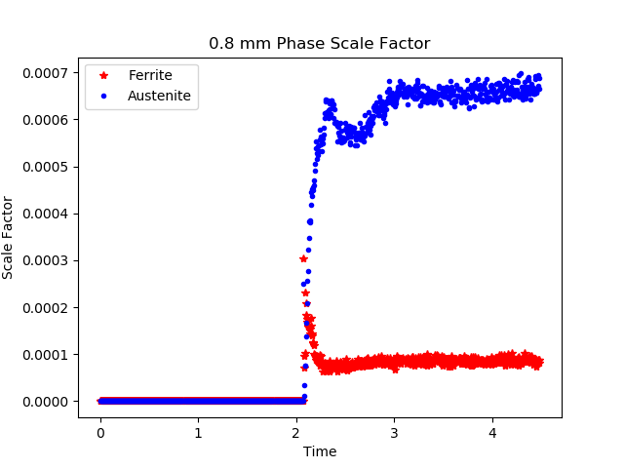
\includegraphics[width=1\linewidth]{raw_scale_factors}
	\caption{Raw scale factors for peak intensity for the Austenite and Ferrite phases in 308L Stainless Steel at a measurement location of 0.8mm above the build substrate. The peak intensity is initially zero because only scattering through the liquid phase was observed.}
	\label{scale}
\end{figure}

The strains calculated from Equation \ref{strain} were used with Equation \ref{zeros} to quantify and calculate the temperature during solidification. Fits of the temperature at each location can be seen in Figure \ref{temp}. The first temperature measurements at 0.4mm are observed just below 1700K which corresponds to 1426$^\circ$ C. This is almost exactly the liquidus temperature of SS 308L. Some of the locations, such as 0.8mm and 1.2mm are slightly lower, in the 1300$^\circ$ C region. The exponential decay of the temperature indicates a changing cooling rate with time, with the rate of temperature change after 1s slowing down considerably. This is consistent with the solidification dynamics that were observed `by eye' during the experiment. The final temperature recorded -- the last data points on Figure \ref{temp} -- was 26$^\circ$ C. 

\begin{figure}
	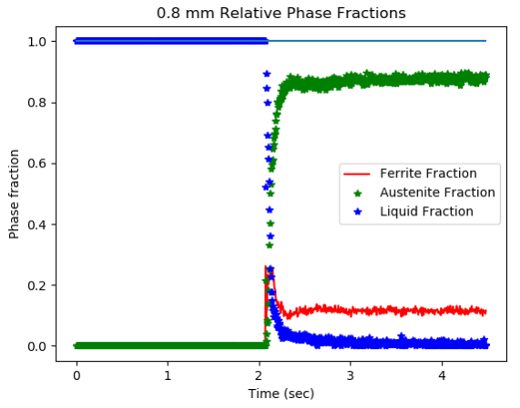
\includegraphics[width=1\linewidth]{converted_liq_phase_fraction}
	\caption{Phase fractions of the liquid, Austenite, and Ferrite phases during solidification at a location of 0.8mm above the build substrate. Initially, the sample is entirely liquid. A rapid transition from the liquid to solid phases occurs, followed by a slow drop off in the liquid fraction until it eventually reaches 0.}
	\label{phasefraction}
\end{figure}

\begin{figure}
	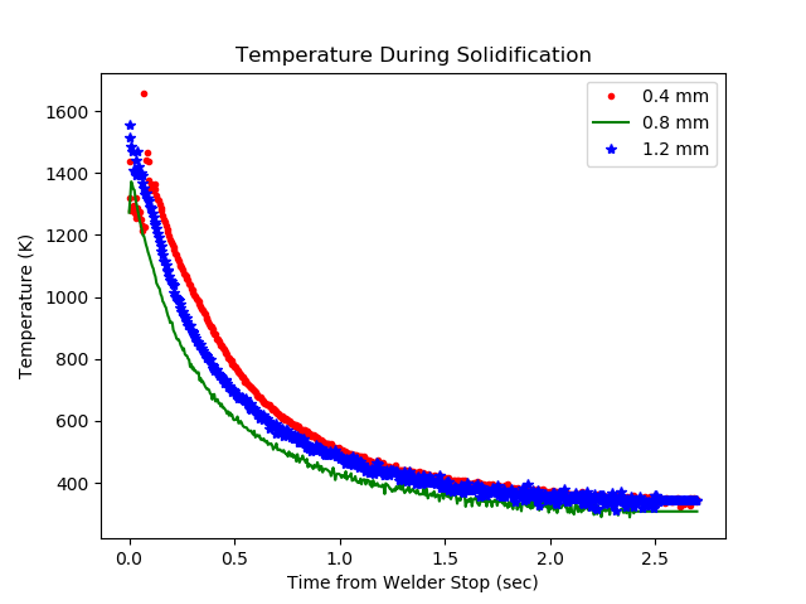
\includegraphics[width=1\linewidth]{converted_SS_temp}
	\caption{Temperature measurements made using Equations \ref{strain} and \ref{touloukian} for all measurement locations.}
	\label{temp}
\end{figure}


\section{Discussion}
The phase fraction measurement shown in Figure \ref{phasefrac} qualitatively agrees with the dynamics expected from a rapidly solidifying weld. The measurement defined in Equation \ref{phasefrac} can be considered a first order fit as it ignores many of the physics of solidification of a material. However, the results it produced are good for such a first order fit. The region of the weld being fit -- that is, the diffracted volume --  is small relative to the size of the bead. Therefore the phase fractions shown in Figure \ref{phasefrac} should be considered as phase fractions only for that small volume of the sample. The fact that the liquid phase did not immediately trend to zero could be a source of error in the measurement. Since other characterization techniques were not used it is not immediately clear whether or not liquid still existed in the sample after 2s, or if another source of amorphous scattering was present, or if this is an artifact of the measurement technique. 

The measurement of temperature found from the sample is considered a great success as the boundaries on the measurement line up very well with the liquidus and solidus of the material. The variations in the starting temperature at each location could be due to several factors. First of all, as shown in Figure \ref{EBSD} there is considerable scatter in the grain sizes spatially across the sample. Certain regions of measurement may have had better grain statistics than others. Regions with more diffracting grains would have better resolution in a Rietveld refinement of peaks because more scattering grains in a fully integrated image results in greater resolution of the peak. Low-resolution peaks have worse weighted residuals in Rietveld refinement.

Another source of error in the temperature measurement would be intergranular stresses. Additional stresses on the sample other than temperature lead to additional strains on diffraction peaks, thus nullifying the assumption that strain is only due to temperature change. The composition of the phases was assumed to be homogenous. If alloys partitioned selectively to one phase over another then their unit cells may have shrunk or grown, adding another source of observed strain on the sample. However, this is not typically observed in CMT welded SS 308L. Furthermore, both phases are cubic phases and so intergranular stresses are expected to be minimized, whereas a sample containing a cubic and non-cubic phase may have had lattice mismatches at the grain boundary. 

The success of the first order fit using Touloukian's model poses opportunities for further characterization of important manufacturing phenomenon such as wire feed additive manufacturing. Models of the additive manufacturing process need to be validated on experimental data which can be relied upon to present accurate measurements of temperature and phase fractions in the sample. While the phase fraction calculations agree with expected behavior qualitatively, further work needs to be done to verify the measurement using other techniques. At the present time, the authors are unaware of other methods for performing this quantification. It may be possible to use calculation of cooling rate from the temperatures with a thermodynamic model to see if the rate of change of the phases accurately matches model predictions.

\section{Conclusion}
Cold metal transfer welded stainless steel 308L was studied and characterized in situ using high energy X-ray diffraction. A monochromatic X-ray beam was shone on samples of SS 308L as they solidified from liquid through solid-solid phase transformations. The phase fractions of the liquid, ferrite, and austenite phases were measured using a new method of calculating phase fractions from the background amorphous scattering of the liquid phase. Lattice strains on the austenite phase were characterized through cooling. The strains calculated were then fit using a model of SS 308L strain as a function of temperature in order to characterize temperatures in the welds during cooling. The temperatures measured accurately predicted the solidification behavior of the samples as evidenced by the close match between initially observed temperatures and the liquidus of the material. This technique can be used for measuring and characterizing important manufacturing phenomenon such as additive manufacturing.

\bibliography{ssbib.bib}
\end{document}
